\documentclass[QCM, noCustomPackages]{UPSTI_Document}
\usepackage{listings}
\usepackage{lstautogobble}
\usepackage{hyperref}
\usepackage{fontawesome}
\usepackage{multirow}
\usepackage{multicol}
\usepackage{currfile}
\usepackage{pdfpages}
\usepackage{placeins}
%\usepackage{pdftricks}




% \begin{psinputs}
%     \usepackage{pstricks}
%     \usepackage{pstricks-add}
%     \usepackage{pst-eucl}
%     \usepackage{color}
%     \usepackage{pstcol}
%     \usepackage{pst-plot}
%     \usepackage{pst-tree}
%     \usepackage{pst-eps}
%     \usepackage{multido}
%     \usepackage{pst-node}
%     \usepackage{pst-eps}
% \end{psinputs}

\definecolor{vert}{rgb}{0.0, 0.5, 0.0}

\newlength{\iconeHeight}
\setlength{\iconeHeight}{15pt}

\newcommand{\UPSTIvariante}{2}


\newlist{todolist}{itemize}{2}
\setlist[todolist]{label=$\square$}
\input{../../../preamble_semestre.tex}
\discipline{Programmation Orientée Objet}
\edef\CurrentFileDir{\currfiledir} 
\graphicspath{{\CurrentFileDir figures/}}

\newcommand{\UPSTIsource}{Certaines images proviennent du site freepics.com}
\newcommand{\UPSTItitreEnTete}{POO}

%%% Définition du langage ST %%%
%New colors defined below
\definecolor{codegreen}{rgb}{0,0.6,0}
\definecolor{codegray}{rgb}{0.5,0.5,0.5}
\definecolor{codepurple}{rgb}{0.502,0.502,0.0}
\definecolor{backcolour}{rgb}{0.95,0.95,0.95}

\lstdefinelanguage{ST}
{
	morekeywords={
	case,of,if,then,end_if,end_case,super,function_block,extends,var,implements,
	constant, byte,,end_var,var_input, real,bool,var_output,
	dint,udint,word,dword,array, of,uint,not,adr, program, for, end_for, while, do, end_while, repeat, end_repeat, until, to, by, else, elsif, var_in_out,interface,method,property
	},
	otherkeywords={
		:, :=, <>,;,\,.,\[,\],\^,1,2,3,4,5,6,7,8,9,0,TRUE, FALSE, \{attribute,  \'hide\'\}
	},
	keywords=[1]{
		case,of,if,then,end_if,end_case,super,function_block,extends,var,implements,
		constant, byte,,end_var,var_input, real,bool,var_output,
		dint,udint,word,dword,array, of,uint,not,adr, :, :=, <>,;,\,.,\[,\],\^,program, for, end_for, while, do, end_while, repeat, end_repeat, until, to, by, else, elsif, var_in_out,interface,method,property
	},
	keywordstyle=[1]\color{blue},
	keywords=[2]{
		1,2,3,4,5,6,7,8,9,0, TRUE, FALSE
	},
	keywordstyle=[2]\color{codepurple},
	keywords=[3]{
		\{attribute,  \'hide\'\}
	},
	keywordstyle=[3]\color{codegray},
	sensitive=false,
	morecomment=[l]{//}, 
	morecomment=[s]{(*}{*)},
	morestring=[b]{"},
	morestring=[b]{'}
}

\lstset{
	language={ST},
	backgroundcolor=\color{backcolour},
	commentstyle=\color{codegreen}\textit,
	keywordstyle=\color{blue},
	numberstyle=\tiny\color{codegray},
	stringstyle=\color{codepurple},
	basicstyle=\ttfamily\scriptsize,
	breakatwhitespace=false,         
	breaklines=true,                 
	captionpos=b,                    
	keepspaces=true,                 
	numbers=left,                    
	numbersep=5pt,                  
	showspaces=false,                
	showstringspaces=false,
	showtabs=false,                  
	tabsize=2
}
%\lstMakeShortInline[columns=fixed]~
\newcommand{\UPSTItitre}{Automatisation d'une cellule de palettisation}
\newcommand{\UPSTInumero}{1}


\documentVersion{E}

\newcommand{\UPSTImessage}{test} 
\setdefaultgroupmode{fixed}
\setgroupmode{cours}{withoutreplacement}


\newcommand{\sujet}{
\exemplaire{1}{%
\renewcommand{\UPSTImessage}{\champnom{\nom{} \prenom{} - Groupe \tp{}}} 
\newcommand{\UPSTInumeroVersion}{55 min}
\UPSTIbuildPage
\setcounter{figure}{0}
\setcounter{table}{0}
%%% debut de l'en-tête des copies : 

% \begin{center}
% \noindent{}\fbox{\vspace*{3mm}
%          \champnom{\Large\bf\nom{} \prenom{} - \id{}}\normalsize{}% 
%           \vspace*{3mm}
%       }
% \end{center}

\section{Présentation du système}

Vous travaillez sur une cellule d'\textbf{ouverture et de vidage de cartons}. Elle est utilisée pour vider automatiquement des cartons contenant un produit connu (par exemple, des sachets) sur un convoyeur spécialisé.

Le système est composé de plusieurs sous-systèmes :
\begin{itemize}
    \item \textbf{Un convoyeur d'alimentation} qui achemine les cartons fermés vers la zone de traitement.
    \item \textbf{Un robot 6 axes} muni d'une pince de préhension. 
    \item \textbf{Ladite pince de préhension} : 
    \begin{itemize}
        \item Permet de saisir un carton,
        \item Est équipée de deux paires de bloqueurs permettant de maintenir les volets du carton ouverts.
    \end{itemize}
    \item \textbf{Un poste de découpe}, équipé d’un actionneur de lame, qui découpe le ruban adhésif fermant le carton.
    \item \textbf{Un poste d'ouverture} permettant de soulever les volets du carton à l’aide de vérins.
    \item \textbf{Un poste de vidage} où le carton est retourné et vidé.
    \item \textbf{Un convoyeur de vidage} qui transporte le contenu du carton vers une station aval.
\end{itemize}

Le système fonctionne de manière cyclique selon les étapes suivantes :
\begin{enumerate}
    \item Le robot saisit un carton sur le convoyeur d'alimentation.
    \item Il le présente au poste de découpe pour sectionner le ruban adhésif.
    \item Il le présente ensuite au poste d'ouverture :
    \begin{itemize}
        \item Les grands volets sont soulevés par le poste d'ouverture,
        \item Le robot les maintient ouverts avec ses bloqueurs,
        \item Le robot effectue une rotation pour exposer les petits volets,
        \item Ceux-ci sont également soulevés, puis maintenus ouverts.
    \end{itemize}
    \item Le carton est ensuite amené au poste de vidage :
    \begin{itemize}
        \item Une plaque métallique se positionne devant l’ouverture du carton,
        \item Le robot retourne le carton, le contenu étant retenu par la plaque,
        \item Il effectue une translation pour déverser le contenu sur le convoyeur,
        \item Un vérin pneumatique pousse le produit restant sur le convoyeur.
    \end{itemize}
\end{enumerate}

\section*{Objectif du devoir}

Ce devoir porte sur la \textbf{modélisation orientée objet} et la \textbf{programmation} du système de préhension. Il se concentre particulièrement sur :

Vous utiliserez les conventions de nommage et les structures proposées à l’IUT. Le raisonnement objet et la capacité à structurer proprement votre code seront des éléments d’évaluation essentiels.

\pagebreak

\section{Conception de la classe \textit{CPincePrehension}}
\label{sec:pince_prehension}

\begin{center}
    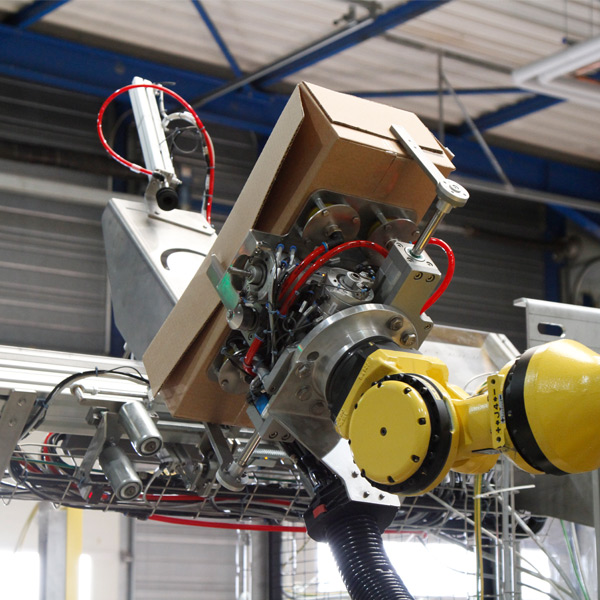
\includegraphics[width=0.7\textwidth]{figures/prehenseur.jpg}
\end{center}

On s'intéresse ici à la modélisation de la pince de préhension du robot. Cette pince est utilisée pour saisir et maintenir les cartons ouverts pendant le processus de vidage.
\subsection*{Description de la pince de préhension}
La pince de préhension est équipée d'un système de préhension par ventouses et de deux paires de bloqueurs.

Le \textbf{système de préhension} par ventouses permet de saisir le carton en appliquant une pression négative pour créer une adhérence. Il est piloté à l'aide d'un distributeur pneumatique qui contrôle l'aspiration et la libération des ventouses. Un capteur de pression est utilisé pour vérifier si le carton est correctement saisi.

Pour les bloqueurs de volets (au nombre de 4), on propose d'utiliser des vérins roto-linaires. Ce sont des vérins permettant une translation linéaire et une rotation. Ils sont utilisés pour maintenir les volets du carton ouverts pendant le processus de vidage. Chaque paire de bloqueurs est contrôlée par un vérin distinct, permettant ainsi de maintenir les volets en position ouverte.


Les questions suivantes portent sur la station d'alimentation.\\
\subsection{Classe \textit{CVerinBlocage}}
\restituegroupe{partie1}
\pagebreak
\subsection{Classe \textit{CPincePrehension}}
On considère que le système de ventouses est décrit par une classe \textbf{CPrehenseur} pouvant recevoir les missions suivantes :

\begin{itemize}
    \item \textbf{Saisir} : Permet de saisir un carton en appliquant une pression négative.
    \item \textbf{Relâcher} : Permet de relâcher le carton en arrêtant l'aspiration.
\end{itemize}

Ses état de sorties sont : 
\begin{itemize}
    \item \textbf{Saisi} : Indique que le carton est correctement saisi.
    \item \textbf{Relâché} : Indique que le carton a été relâché.
    \item \textbf{Erreur} : Indique un problème lors de la saisie ou du relâchement.
\end{itemize}



\restituegroupe{superviseur}
\pagebreak
\section{Questions de cours}
\restituegroupe[2]{cours}
\clearpage

}
}
\begin{document}



\AMCassociation{\id}
\AMCrandomseed{1237893}

\element{cours}{
    \begin{question}{q01}
        Rappeler ce que signifie qu'une classe est dérivée d'une autre.\\
        \evaluationProfLignes{2}{2}
    \end{question}
}

\element{cours}{
    \begin{question}{q02}
        Représenter graphiquement la structure interne d'un objet de commande.\\
        \evaluationProfLignes{2}{5}
    \end{question}
}

\element{cours}{
    \begin{question}{q03}
        Quand utiliser le pointeur \lstinline|SUPER| ?\\	
        \evaluationProfLignes{2}{2}    
    \end{question}
}

\element{cours}{
    \begin{question}{q03}
        Rappeler le type de POU utilisé pour implémenter une classe dans l'univers CodeSys. Justifier ce choix.\\
        \evaluationProfLignes{2}{2}    
    \end{question}
}

\element{cours}{
    \begin{question}{q04}
        Expliquer la différence entre les accesseurs \lstinline|get| et \lstinline|set|.\\
        \evaluationProfLignes{2}{2}
    \end{question}
}

\element{cours}{
    \begin{question}{q05}
        Déclarer un tableau de 6 booléens. 
        \evaluationProfLignes{2}{2}
    \end{question}
}

\element{cours}{
    \begin{question}{q06}
        Rappeler la définition d'un système temps réel.
        \evaluationProfLignes{2}{2}
    \end{question}
}

\element{cours}{
    \begin{question}{q07}
        Déclarer une structure \lstinline|TVehicule| comportant deux membres : 
        \begin{itemize}
            \item un entier \lstinline|m_nbrDeRoue|, 
            \item un réel \lstinline|m_vitesseMax|.
        \end{itemize}
        \evaluationProfLignes{2}{2}
    \end{question}
}



\element{partie1}{
    \begin{question}{verin-io}
        \evaluationProf[2]\\
        A partir de la description précédente, de la vidéo et de la documentation du vérin roto-linéaire fournie, proposer une liste des entrées et sorties nécessaires pour piloter un vérin de blocage.\\
        Compléter la section GVL avec vos réponse. Donner des adresses compatibles avec le type utilisé. \\
    \end{question}
}

\element{partie1}{
    \begin{question}{verin-missions}
        \evaluationProf[2]\\
        A partir de la vidéo et de la description du système, proposer une liste des missions que doit pouvoir réaliser un vérin de blocage roto-linéaire. Vous répondrez en déclarant le type de données \lstinline{TMissionVerinBlocage} dans votre programme.
    \end{question}
}

\element{partie1}{
    \begin{question}{verin-etats}
        \evaluationProf[2]\\
        Proposer la déclaration d'un type de données adaptées pour décrire les états possibles d'un vérin de blocage.\\
    \end{question}
}

\element{partie1}{
    \begin{question}{verin-declaration}
        \evaluationProf[2]\\
        A partir des questions précédentes, déclarer la classe \lstinline{CVerinBlocage} et compléter son contexte.\\
        \textit{Votre réponse contiendra la déclaration de la classe, les variables d'entrées, de sorties ainsi que les variables représentant les états et les missions.}\\
    \end{question}
}

\element{partie1}{
    \begin{question}{getSet}
        \evaluationProf[2]\\
        Donner l'implémentation des propriétés permettant d'accéder aux missions et états de la classe.\\
        \textit{Vous indiquerez également celles qui vous semblent inutiles en justifiant votre réponse.}
    \end{question}
}

\element{partie1}{
    \begin{question}{verin-corps}
        \evaluationProf[2]\\
        Proposer le contenu de la méthode permettant l'exécution de la mission reçue. (\textit{MExecutionMission})\\
    \end{question}
}

\element{partie1}{
    \begin{question}{setoutput}
        \evaluationProf[2]\\
        Proposer le corps de la fonction permettant de mettre à jour les sorties de la station d'alimentation.
    \end{question}
}

\element{partie1}{
    \begin{question}{verin-appel}
        \evaluationProf[2]\\
        Appeler un bloc fonctionnel \lstinline{oStation} de type \lstinline{CStationAlimentation} dans le programme principal.
    \end{question}
}



\pagebreak
\element{partie1}{
    \begin{question}{verin-missions-2}
        Proposer un grafcet de la mission permettant le blocage d'un volet.\\
        \evaluationProfGrille{2}{14}
    \end{question}
}

\element{superviseur}{
    \begin{question}{pointeurs}
        \evaluationProf[2]\\
        Déclarer les membres de la classe \lstinline|CPince| permettant de faire le lien avec les objets qu'elle commande. \\
    \end{question}
}

\element{superviseur}{
    Après un arrêt d'urgence, l'opérateur peut lancer une procédure de reprise (Mode A5). Durant ce mode, la pince recevra une mission d'initialisation. Pour la pince, cette mission consiste en : 
    \begin{itemize}
        \item Relacher le préhenseur, 
        \item Rentrer les vérins de blocage
    \end{itemize}
     \begin{question}{a5}
        \evaluationProf[2]\\
        Dans la méthode \textit{MExecutionMission} de la classe pince, écrire les lignes de code permettant de réaliser cette mission.\\
    \end{question}
}


\def\AMCformQuestion#1{{\sc Question #1 :}}
\csvreader[head to column names,]{etudiants_D.csv}{}{\sujet}
\end{document}


